%%%%%%%%%%%%%%%%%%%%%%%%%%%%%%%%%%%%%%%%%%%%%%%%%%%%%%%%%%%%%%%%%%%
%                            Section 5.1
%%%%%%%%%%%%%%%%%%%%%%%%%%%%%%%%%%%%%%%%%%%%%%%%%%%%%%%%%%%%%%%%%%%%
\chapter{5.1 Systems of Linear Equations in 2 Variables}
%%%%%%%%%%%%%%%% SECTION HEADER %%%%%%%%%%%%%%%%
\rhead{1}
\lhead{Systems of Linear Equations in 2 Variables}
%%%%%%%%%%%%%%%%%%% START %%%$%%%%%%%%%%%%%%%%%
\section{Introduction}
Imagine you go to the store and buy 1 Tilapia fish and 1 Salmon fish and they cost $\$12$. The next day, you go to the same store and buy 2 Tilapia fish and 1 Salmon fish. This time your total is $\$17$. The question is how we can find the price for each fish. \\
Let $x$ the price of 1 Tilapia fish and $y$ the price of 1 Salmon fish. Therefore, translating from English to mathematics, we would get:
\[
\begin{dcases}
\text{1 Tilapia}+\text{1 Salmon}= 12 \\[1ex]
\text{2 Tilapia}+\text{1 Salmon}= 17
\end{dcases}
\quad\implies\quad
\begin{dcases}
1x+1y=12 \\[1ex]
2x+1y=17
\end{dcases}
\]
We obtain two equations with two unknowns. These two equations are happening at the same time. This is called a system of equations with 2 unknowns.\\
In general, if we have $n$ number of linear equations, $n>2$, each with $n$ number of unknowns, which are occurring at the same time, then we have a system of linear equations. For example, following equations create a system of linear equation in three variables,
		\begin{empheq}[left={\empheqlbrace}]{align*}
				x-2y +z &=5 \\
				2x-5y -3z&=9 \\
				x+4y -2z&=-2
			\end{empheq} 
In this section, we will focus on a system that has only two equations with 2 unknowns. The \textbf{solution for a system of linear equations} is an ordered pair that satisfies \textbf{both equations} in the system.
% =================== EXAMPLE 1
\begin{example}
Determine whether $(-3, 4)$ is a solution to the following system.
		\begin{empheq}[left={\empheqlbrace}]{align*}
				2x+2y &=6\\
				3x-4y &=7	
		\end{empheq}
\end{example}
%
We will begin by substituting $(-3, 4)$ into the first equation to see whether the  ordered pair is a solution to the first equation	
		\begin{align*}
			2(-3)-2(4) &\stackrel{?}{=} 5 \\
			-6 +12 &\stackrel{?}{=}	5 \\
			5 &=5 \qquad \checkmark
		\end{align*}
Likewise, we will substitute $(-3, 4)$ into the second equation. Thus,
		\begin{align*}
			3(-3)-4(4) &\stackrel{?}{=} 5 \\
			-9 -16 &\stackrel{?}{=}	5 \\
			-25 &=5 \qquad \xmark
		\end{align*}
Ordered pair $(-3, 4)$ satisfies the first equation but not the second equation. Therefore, this ordered pair is not the solution of the system. 
% ============== NOTE
\begin{note}
    As you observed in previous example, the ordered pair should satisfies both equations. If it only satisfies one of them, it is not the solution of our system.
\end{note}
% ================ SECTION
\section{Solving a system of linear equation}
There are many ways to find the solution for a system of linear equations. We will only discuss 3 major methods in this section:
\begin{itemize}
	\item Graphing
	\item Substitution
	\item Addition (or Elimination)
\end{itemize}
% ========== SUBSECTION
\subsection{Graphing method}
Each equation in a system of equation with two variables is representing a line in the $xy$-plane. If you graph each of them, there will be three possibilities:
\begin{enumerate}[I.]
	\item \textbf{Two lines intersect each other at one point:} if two lines intersect, the point of intersection lies on both lines. Thus, the point of intersection is our only solution. Such a system is said to have a unique solution.
		\begin{figure}[H]
			 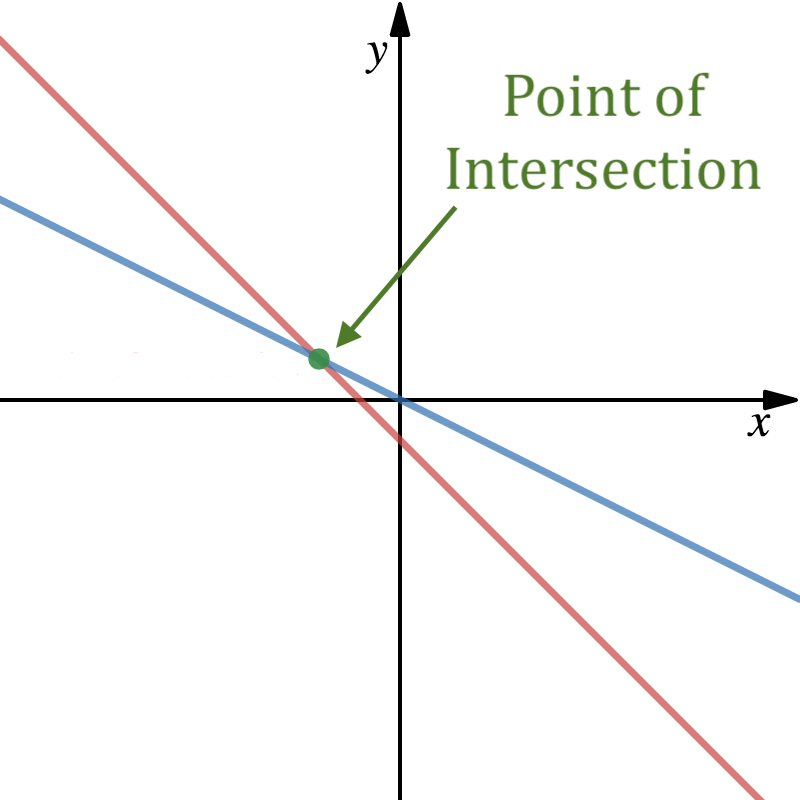
\includegraphics[width=5cm]{pics/line_intersect.png}
			 \centering
			 \caption{Intersection of two lines.}
			 \label{fig:line_intersect}
		\end{figure}
	\item \textbf{Two lines don’t intersect each other at all:} This happens when two lines are parallel to each other. Since they don’t intersect each other, we do not have any solution. Such a system is said to be inconsistent.
		\begin{figure}[H]
			 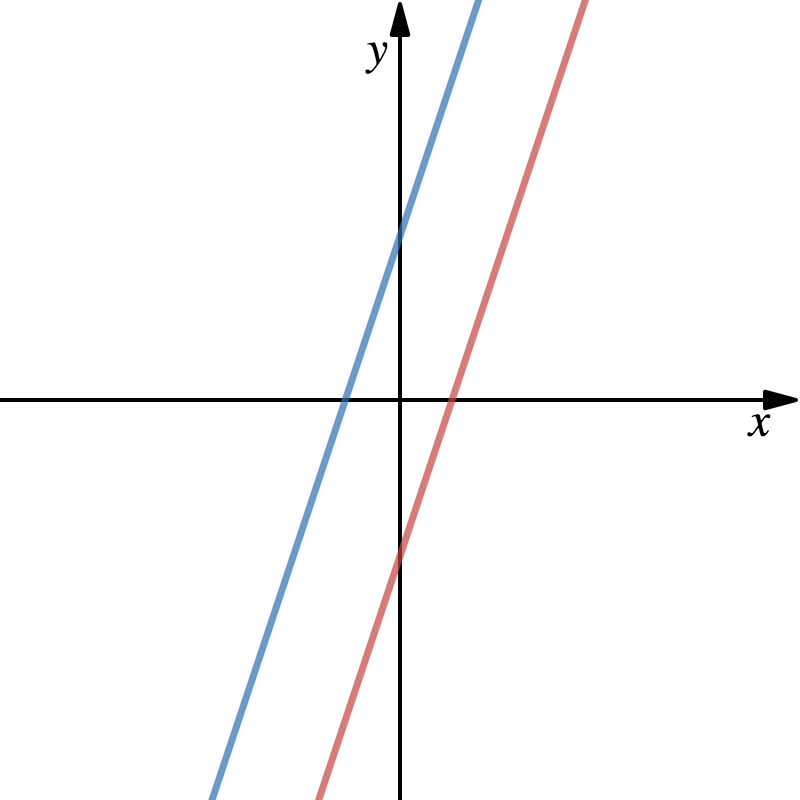
\includegraphics[width=5cm]{pics/line_parallel.png}
			 \centering
			 \caption{Parallel lines.}
			 \label{fig:line_parallel}
		\end{figure}
	\item \textbf{Two lines are actually same line:} Another possibility is that when we graph each equation in the system, we obtain one line. In such a case, there is an infinite number of solutions. Because any point that lies on the first line will also lie on the second line. Such a system is said to have dependent equations.
		\begin{figure}[H]
			 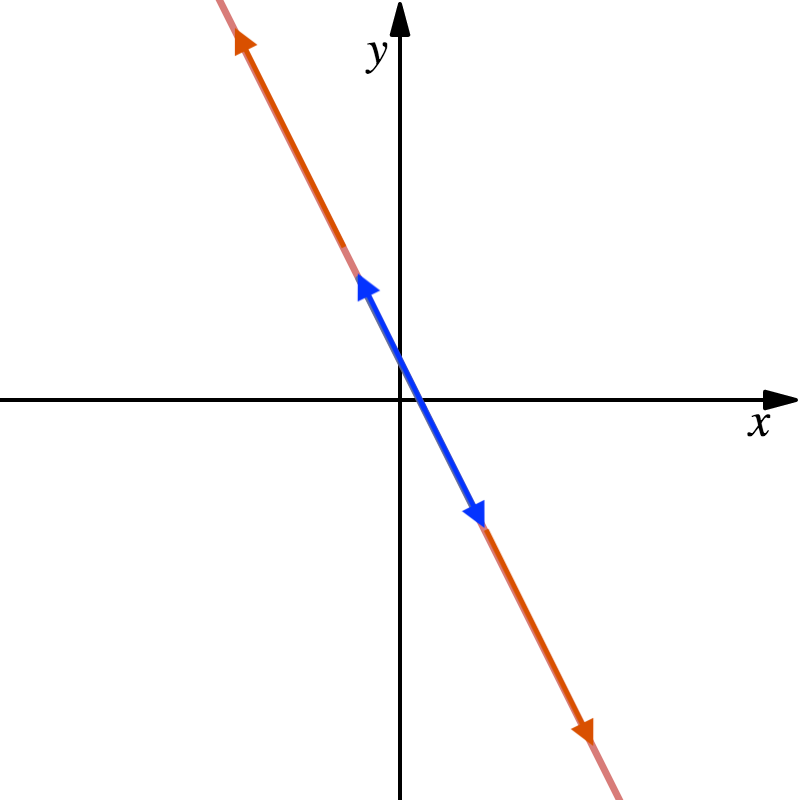
\includegraphics[width=5cm]{pics/line_same.png}
			 \centering
			 \caption{Same lines.}
			 \label{fig:line_same}
		\end{figure}
\end{enumerate}
% =========== SUBSECTION
\subsection{Substitution method}
When solving a system by graphing has several limitations. First, it requires the graph to be perfectly drawn, if the lines are not straight we may arrive at the wrong answer. Second, graphing is not a great method to use if the answer is really large, over $100$ for example, or if the answer is a decimal the that graph will not  help us find, $3.2134$ for example. For these reasons we will rarely use graphing to solve our systems. Instead, an algebraic approach will be used. The first algebraic approach is called substitution.
%
\begin{tcolorbox}[title= Substitution Method,fonttitle=\bfseries,
	                  colframe=blue!70!black,
	                  colback=white]
\begin{enumerate}
    \item	Choose one of the equations and solve for one variable in 
            terms of the other variable.
    \item	Substitute the expression from Step 1 into the other    
            equation. 
    \item	Solve the equation from Step 2. (There will be one equation         with one variable). 
    \item	Substitute the solution from Step 3 into either of the 
            original equations. This will give the value of the other variable.
\end{enumerate}
\end{tcolorbox}
%
\textbf{Common Mistakes to Avoid:}
\begin{itemize}
    \item	Remember that a system of linear equations is not completely         solved until values for both $x$ and $y$ are found. To avoid         this mistake, write all answers as an ordered pair.
    \item	Remember that all ordered pairs are stated with the
            $x$ variable first and the $y$ variable second; namely, $(x, y)$. 
    \item	If the first equation is used to solve for the variable,
            you must substitute it into the second equation. Otherwise, this will incorrectly lead to the statement $0 = 0$.
\end{itemize}
% ================== EXAMPLE 2
\begin{example}
Solve.
		\begin{empheq}[left={\empheqlbrace}]{align*}
				2x+y &=5\\
				3x+2y &=-8	
		\end{empheq}
\end{example}
%
Notice, the first equation can be solved easily for $y$, giving us
		\begin{align*}
			2x+y =5&    &   &\text{Subtract $2x$ from both sides} \\
		    \boxed{y=5-2x}&	    &   &\text{$y$ in terms of other veriable}
		\end{align*}
This is what we will now substitute into the $y$ variable in our second equations. This gives us:
		\begin{align*}
			3x+2(5-2x) =-8& 	&&\text{Distribute}\\
			3x+10-4x = -8&      &&\text{Combine like terms}\\
			10-x =-8&       	&&\text{Subtract 10 from both sides}\\
			-x = -18&	        &&\text{Divide by -1}\\
			x =18&              &&\text{Our $x$}
		\end{align*}
Next, we need to find the value of our $y$ variable by substituting $x=18$ into either equation. Since we already know that $y=5-2x$, substituting in this equation gives us:
		\begin{align*}
			y&=5-2(18)\\
			y&=5-36 \\
			y&=-31	
		\end{align*}
So our solution is $(18,-31)$.
% ============== EXAMPLE 3
\begin{example}
Solve.
		\begin{empheq}[left={\empheqlbrace}]{align*}
				2x+3y &=5\\
				x-4y &=6	
		\end{empheq}
\end{example}
%
Notice, the second equation can be solved easily for $x$, so
		\begin{align*}
			x-4y =6&    &   &\text{Add $4y$ to both sides} \\
			\boxed{x=6+4y}&	    &   &\text{$x$ in terms of other variable}
		\end{align*}
We will now substitute this into the $x$ variable in our first equation
		\begin{align*}
			2(6+4y)+3y =5&  	&&\text{Distribute}\\
			12+8y+3y = 5&       &&\text{Combine like terms on LHS}\\
			12+11y =5&	        &&\text{Subtract 12 from both sides}\\
			11y = -7&	        &&\text{Divide by 11}\\
			y =\frac{-7}{11}    &&\text{Our $y$}
		\end{align*}
Finally, we need to solve for $x$ variable by substituting $y=-\frac{7}{11}$ into one of our equations. Since we already know that $x=6+4y$ substituting into this equation, giving us 
		\begin{align*}
			x&=6+4\left(\frac{-7}{11}\right)\\
			x&=6-\frac{28}{11} \\
			x&=\frac{38}{11}
		\end{align*}
So our answer is $\displaystyle \left(\frac{38}{11},\frac{-7}{11}\right)$.
% ================ NOTE
\begin{note}
During solving a system with two variables, if you get a false statement, means that we have no solution. On the other hand, if you reach to a true statement, like $0=0$, thus you have infinite solutions.
\end{note}
% ============== EXAMPLE 4
\begin{example}
Solve.
		\begin{empheq}[left={\empheqlbrace}]{align*}
				2x-y &=3\\
				-6x+3y &=9	
		\end{empheq}
\end{example}
%
Notice, the first equation can be solved quickly for $y$, 
		\begin{align*}
			2x-y =3&    &   &\text{Subtract $2x$ from both sides} \\
			-y=3-2x&    &   &\text{Divide both sides by $-1$}\\
			\boxed{y=-3+2x}&    &   &\text{$y$ in terms of other variable}
		\end{align*}
We now substitute this into the $y$ variable in our second equation
		\begin{align*}
			-6x+3(-3+2x) =9&		&&\text{Distribute}\\
			-6x-9+6x = 9&           &&\text{Combine like terms}\\
			-9 =9&\ \,\xmark    	&&\text{A false statement}\\
		\end{align*}
Since this is a false statement, the system is inconsistent. Therefore, there is no solution.
% ============= SUBSECTION
\subsection{Elimination method}
When solving systems, we have found that graphing is very limited when solving equations. We then considered a second method known as substitution. This is probably the most used idea in solving systems in various areas of algebra. However, substitution can get ugly if we don’t have a lone variable. This leads us to our second method for solving systems of equations. This method is known as either Elimination or Addition.
\begin{tcolorbox}[title=Elimination Method, fonttitle=\bfseries,
	                  colframe=blue!70!black,
	                  colback=white]
\begin{enumerate}
    \item	Line up the variables and constants.
    \item	Multiply one or both equations by appropriate numbers (use 
            LCM if you cannot find that magic numbers) so that the coefficient of one of the variables are opposites.
    \item	Add the two equations from step 2 to remove one of the 
            variable
    \item 	Solve the resulting equation for the remaining variable
    \item 	Substitute the value you found from previous step into one
            of the original equations and find the other variable.
\end{enumerate}
\end{tcolorbox}
%
\textbf{Common Mistakes to Avoid:}
\begin{itemize}
    \item	Remember that a system of linear equations is not completely         solved until values for both $x$ and $y$ are found. To avoid         this mistake, write all answers as ordered pairs. 
    \item	Remember that all ordered pairs are stated with the
            $x$ variable first and the $y$ variable second; namely, $(x, y)$.
\end{itemize}
% ============ EXAMPLE 5
\begin{example}
Solve 
		\begin{empheq}[left={\empheqlbrace}]{align*}
				6x-5y &=25\\
				4x+15y &=13	
		\end{empheq}
\end{example}
%
If we multiply the first equation by $3$ and leave the second equation alone, we will eliminate $y$.
\[
\begin{dcases}
\textcolor{red}{3(}6x-5y\textcolor{red}{)} &=\textcolor{red}{3(}25\textcolor{red}{)} \\[1ex]
4x+15y &=13	
\end{dcases}
\quad\implies\quad
\begin{dcases}
18x-15y &=75 \\[1ex]
4x+15y &=13	
\end{dcases}
\]
%
Add these two equations together we get
\begin{align*}
18x \cancel{{}-15y} &= 75 \\
4x \cancel{{}+ 15y} &= 13 \\[-.2cm]
\cline{1-2}
22x &= 88 \\
x &= 4
\end{align*}
Now we must find the value for $y$ by substituting $x=4$ into one of the two original equations. Substituting into the first equation gives us:
		\begin{align*}
			6(4)-5y &=	25\\
			24-5y &= 25\\
			-5y &= 1\\
			y &= -\frac{1}{5}	
		\end{align*}
So the answer is $\displaystyle (4,-\frac{1}{5})$
% ============ EXAMPLE 6
\begin{example}
Solve 
		\begin{empheq}[left={\empheqlbrace}]{align*}
				8x+9y &=13\\
				6x-5y &=45	
		\end{empheq}
\end{example}
%
To eliminate the $x$ variable, find the LCM of the coefficient of $x$ variables. The LCM of $8$ and $6$ is $24$. To create $24$, we will multiply the first equation by $-3$  and the second equation by $4$. Recall that their coefficient should be opposite. That's why we multiply one of them by $-3$.
\[
\begin{dcases}
\textcolor{red}{-3(}8x+9y\textcolor{red}{)} &=\textcolor{red}{-3(}  13  \textcolor{red}{)} \\[1ex]
\textcolor{red}{4(}6x-5y\textcolor{red}{)} &=\textcolor{red}{4(}    45\textcolor{red}{)}	
\end{dcases}
\quad\implies\quad
\begin{dcases}
	-24x-27y &=-39 \\[1ex]
	24x-20y &=180
\end{dcases}
\]
Add these two equations together yields
\begin{align*}
\cancel{{}-24x} -27y &= -39 \\
\cancel{{}24x} -20y &= 180 \\[-.2cm]
\cline{1-2}
-47y &= 141 \\
y &= -3
\end{align*}
%
Next, we need to find the value for $x$ by substituting $y=-3$ into either of the two original equations. If we substituting into the first equation, we get:
		\begin{align*}
			8x+9(-3) &=	13\\
			8x-27 &= 13\\
			8x &= 40\\
			x &= 5	
		\end{align*}
So the answer is $\displaystyle (5,-3)$
% =============== EXAMPLE 7
\begin{example}
Solve 
		\begin{empheq}[left={\empheqlbrace}]{align*}
				-6x+9y &=12\\
				2x-3y &=-4	
		\end{empheq}
\end{example}
If we multiply the second equation by $3$, we can eliminate $x$
\[
\begin{dcases}
-6x+9y &=12\\[1ex]
\textcolor{red}{3(}2x-3y\textcolor{red}{)} &=\textcolor{red}{3(}    -4\textcolor{red}{)}	
\end{dcases}
\quad\implies\quad
\begin{dcases}
	-6x+9y &=12 \\[1ex]
	6x-9y &=-12
\end{dcases}
\]
When we add these two equations together, we get
\begin{align*}
-6x+9y &=12 \\
6x-9y &=-12 \\[-.2cm]
\cline{1-2}
    0 &= 0
\end{align*}
%
Since we get a true statement, this system is dependent. Therefore, there are an infinite number of solutions.

